\documentclass[14pt,xcolor=pdftex,dvipsnames,table]{beamer}\usepackage[]{graphicx}\usepackage[]{color}
%% maxwidth is the original width if it is less than linewidth
%% otherwise use linewidth (to make sure the graphics do not exceed the margin)
\makeatletter
\def\maxwidth{ %
  \ifdim\Gin@nat@width>\linewidth
    \linewidth
  \else
    \Gin@nat@width
  \fi
}
\makeatother

\definecolor{fgcolor}{rgb}{0.345, 0.345, 0.345}
\newcommand{\hlnum}[1]{\textcolor[rgb]{0.686,0.059,0.569}{#1}}%
\newcommand{\hlstr}[1]{\textcolor[rgb]{0.192,0.494,0.8}{#1}}%
\newcommand{\hlcom}[1]{\textcolor[rgb]{0.678,0.584,0.686}{\textit{#1}}}%
\newcommand{\hlopt}[1]{\textcolor[rgb]{0,0,0}{#1}}%
\newcommand{\hlstd}[1]{\textcolor[rgb]{0.345,0.345,0.345}{#1}}%
\newcommand{\hlkwa}[1]{\textcolor[rgb]{0.161,0.373,0.58}{\textbf{#1}}}%
\newcommand{\hlkwb}[1]{\textcolor[rgb]{0.69,0.353,0.396}{#1}}%
\newcommand{\hlkwc}[1]{\textcolor[rgb]{0.333,0.667,0.333}{#1}}%
\newcommand{\hlkwd}[1]{\textcolor[rgb]{0.737,0.353,0.396}{\textbf{#1}}}%

\usepackage{framed}
\makeatletter
\newenvironment{kframe}{%
 \def\at@end@of@kframe{}%
 \ifinner\ifhmode%
  \def\at@end@of@kframe{\end{minipage}}%
  \begin{minipage}{\columnwidth}%
 \fi\fi%
 \def\FrameCommand##1{\hskip\@totalleftmargin \hskip-\fboxsep
 \colorbox{shadecolor}{##1}\hskip-\fboxsep
     % There is no \\@totalrightmargin, so:
     \hskip-\linewidth \hskip-\@totalleftmargin \hskip\columnwidth}%
 \MakeFramed {\advance\hsize-\width
   \@totalleftmargin\z@ \linewidth\hsize
   \@setminipage}}%
 {\par\unskip\endMakeFramed%
 \at@end@of@kframe}
\makeatother

\definecolor{shadecolor}{rgb}{.97, .97, .97}
\definecolor{messagecolor}{rgb}{0, 0, 0}
\definecolor{warningcolor}{rgb}{1, 0, 1}
\definecolor{errorcolor}{rgb}{1, 0, 0}
\newenvironment{knitrout}{}{} % an empty environment to be redefined in TeX

\usepackage{alltt}

% Specify theme
\usetheme{Madrid}
% See deic.uab.es/~iblanes/beamer_gallery/index_by_theme.html for other themes
\usepackage{caption}
\usepackage[comma, sort&compress]{natbib}
\usepackage{tikz}
\usepackage{graphicx}
\graphicspath{{./Figures/}}
\usepackage{amsmath}
\bibliographystyle{agsm}
% Specify base color
\usecolortheme[named=OliveGreen]{structure}
% See http://goo.gl/p0Phn for other colors

% Specify other colors and options as required
\setbeamercolor{alerted text}{fg=Maroon}
\setbeamertemplate{items}[square]

% Title and author information
\title{Trading in Financial Markets}
\author{Rob Hayward}
\IfFileExists{upquote.sty}{\usepackage{upquote}}{}
\begin{document}

\begin{frame}
\titlepage
\end{frame}

\begin{frame}{Outline}
\tableofcontents
\end{frame}


\section{What is trading?}
\begin{frame}{What is trading?}
\begin{itemize}
\item Market-making
\item Proprietary trading
\item Investment 
\end{itemize}
\end{frame}

\begin{frame}{Market-Making}
There is a distinction between the \emph{primary} and \emph{secondary} markets
\pause
\begin{itemize}[<+-| alert@+>]
\item Open-outcry
\item Dealer (bid-ask)
\item Electronic (order-driven)
\end{itemize}
\end{frame}


\begin{frame}{Market-making: Open outcry}
\frametitle{Open Outcry}
\begin{center}
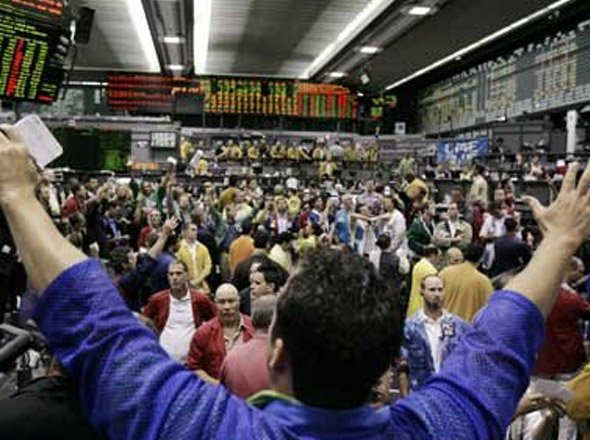
\includegraphics[height = 3.0in]{Open-Out-Cry}
\end{center}
\end{frame}

\begin{frame}{London Metal Exchange}
\begin{center}
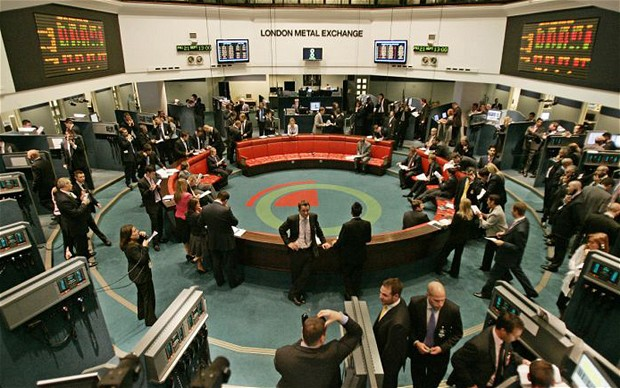
\includegraphics[height = 3.0in]{LME}
\end{center}
\end{frame}


\begin{frame}{Market-making: Dealer}
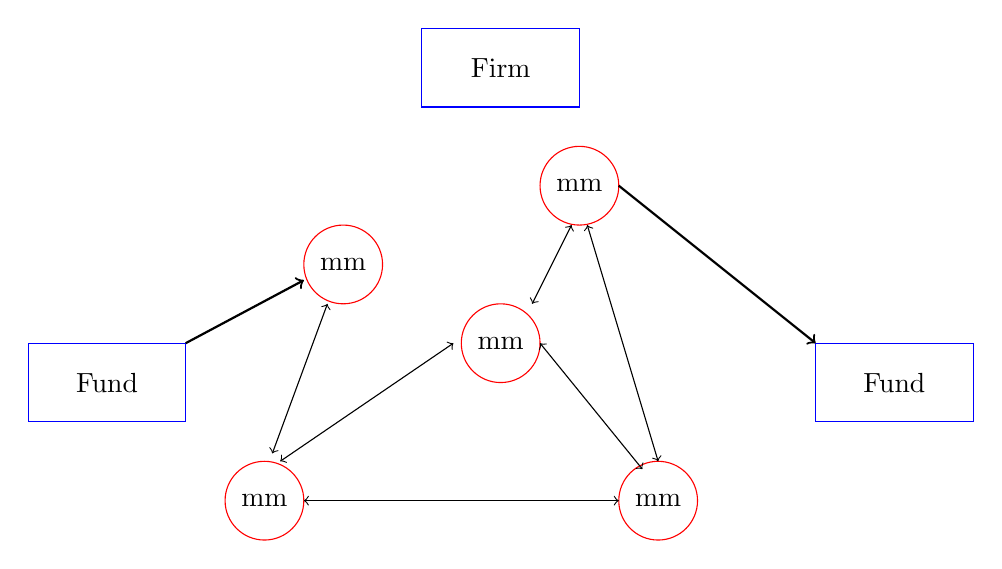
\begin{tikzpicture}[xscale = 1, yscale = 1]
\draw [blue] (1,1) rectangle (3, 2);
\node at (2, 1.5) {Fund};
\draw [blue] (6,5) rectangle (8, 6);
\node at (7, 5.5) {Firm};
\draw [blue] (11,1) rectangle (13, 2);
\node at (12, 1.5) {Fund};
\pause
\draw [red] (5,3) circle [radius = 0.5];
\node at (5, 3) {mm};
\draw [red] (7,2) circle [radius = 0.5];
\node at (7,2) {mm};
\draw [red] (4,0) circle [radius = 0.5];
\node at (4,0) {mm};
\draw [red] (8,4) circle [radius = 0.5];
\node at (8, 4) {mm};
\draw [red] (9,0) circle [radius = 0.5];
\node at (9, 0) {mm};
\pause
\draw [thick] [->] (3,2) -- (4.5,2.8);
\draw [thick] [->] (8.5, 4) -- (11,2);
\pause
\draw [<->] (4.1, 0.6) -- (4.8, 2.5);
\draw [<->] (4.5, 0) -- (8.5, 0);
\draw [<->] (8.8, 0.4) -- (7.5, 2);
\draw [<->] (9, 0.5) -- (8.1, 3.5);
\draw [<->] (4.2, 0.5) -- (6.4, 2);
\draw [<->] (7.4, 2.5) -- (7.9, 3.5);
\end{tikzpicture}
\end{frame}

\begin{frame}{Market making: Dealer: Bid-Ask}
\frametitle{Bid-Ask}
\begin{center}
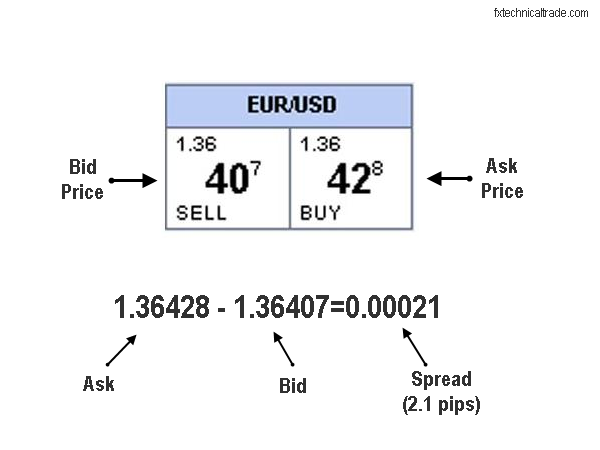
\includegraphics[height = 1.8in, trim = 0 10 0 10]{Bid-Ask}
\end{center}
\end{frame}

\begin{frame}{Electronic order market}
Features of the order-driven market
\pause
\begin{itemize}[<+-| alert@+>]
\item It is more transparent
\item It is standardised
\item Counterparty risk is switched to the exchange
\item Liquidity can be an issue
\end{itemize}
\end{frame}


\begin{frame}{Proprietary trading}
\begin{itemize}[<+-| alert@+>]
\item Using institution's capital 
\item Risk-adjusted return relative to cost of funds
\item Flavours of carry trade
\item Arbitrage opportunities
\end{itemize}
\end{frame}

\begin{frame}{Proprietary trading: Carry trade}
\frametitle{Carry trade}
\begin{center}
\includegraphics[height = 3.1in, width = 4.9in, trim = 45 0 5 85]{yield}
\end{center}
\end{frame}

\begin{frame}{Investment}
\begin{itemize}[<+-| alert@+>]
\item Long term 
\item Managing others' funds
\item Versions of \emph{Value Investment}
\item Asset allocation or security selection
\item Other activities to \emph{enhance} returns
\begin{itemize}
\item Securities lending
\item Currency overlay
\end{itemize}
\end{itemize}
\end{frame}

\section{Institutional features}
\begin{frame}{Institutional features}
\begin{itemize}
\item Commercial banks
\item Investment banks
\item Funds
\item Exchanges
\item Government
\end{itemize}
\end{frame}

\begin{frame}{Commercial banks}
Not a large part of the story, but
\pause
\begin{itemize}[<+-| alert@+>]
\item Cheap and secure funding from 
\begin{itemize}
\item Depositors
\item Central bank
\end{itemize}
\item Controversy over Investment banking-commercial banking link
\item Divergence UK and Continental Europe
\end{itemize}
\end{frame}

\begin{frame}{Investment banks}
Investment banks have become less significant
\pause
\begin{itemize}[<+-| alert@+>]
\item Proportion of market-making to proprietary trading will increase
\begin{itemize}
\item Effect of regulation
\item Effect of funding costs
\end{itemize}
\item See Goldman, JP Morgan and others Q413 results
\begin{itemize}
\item Proportion of M\&A to FICC increased
\item Goldman FICC down 15\% to \$1.7bn
\end{itemize}
\item \emph{The Volcker Rule}
\end{itemize}
\end{frame}

\begin{frame}{Investment banks: The Volcker Rule}
\frametitle{The Volcker Rule}
\begin{center}
\includegraphics[height = 3.1in]{Paulvolcker}
\end{center}
\end{frame}

\begin{frame}{Funds}
A variety of funds and other boutique and specialist financial institutions become more prominent in proprietary trading
\begin{itemize}[<+-| alert@+>]
\item Traditional funds: securities lending
\item Hedge funds
\item Small-scale prop and spec book
\item OSTC 
\item Brighton futures
\end{itemize}
\end{frame}

\begin{frame}{NYSE}
\begin{center}
\includegraphics[height = 3.0in]{NYSE-floor}
\end{center}
\end{frame}

\begin{frame}{Exchanges}
Exchanges have become increasingly important
\pause
\begin{itemize}[<+-| alert@+>]
\item Natural monopolies: network effects
\item Exchanges have shifted from being mutually owned to being public companies
\item Aim to extend monopolistic power from trading to other activities such as settlement and custody
\item Post-crisis regulation aims to push more trading onto exchanges
\end{itemize}
\end{frame}

\begin{frame}{Government}
Mifid 2 is the latest European legislation
\pause
\begin{itemize}[<+-| alert@+>]
\item Rules are a by product of the interaction of 
\begin{itemize}
\item Countries
\item Heads of State, Commission and EU Parliamenrt
\item US and EU
\end{itemize}
\item Main Elements of Mifid 2
\begin{itemize}
\item HFT
\item Commodity position limits
\item Dark pools
\item Exchange-clearing Silos
\end{itemize}
\end{itemize}
\end{frame}

\section{Trading techniques}
\begin{frame}{Trading techniques}
\begin{itemize}
\item Value investment
\item Momentum
\item Contrarianism
\item Carry trade
\item Arbitrage
\item Automation
\end{itemize}
\end{frame}

\begin{frame}{Momentum}
\begin{center}
\includegraphics[height = 3.2in, trim = 40 0 0 90]{aapl}
\end{center}
\end{frame}

\begin{frame}{Momentum 2}
What causes trends?  How can trends be identified and used?  
\pause
\begin{itemize}[<+-| alert@+>]
\item A number of factors may cause momentum
\begin{itemize}
\item \emph{Conservatism} and gradual reaction of people to new information
\item The social element of information or belief
\item Asynchronous trading
\end{itemize}
\item Trading methods used to take advantage of momentum
\begin{itemize}
\item Technical analysis:  trends and moving average
\item Early identification of trend
\item Indications that the trend is ending
\end{itemize}
\end{itemize}
\end{frame}

\begin{frame}{Contrarianism}
Seeks to identify bursting bubbles
\begin{itemize}[<+-| alert@+>]
\item \emph{Representativeness} or \emph{Availability} heuristics
\item Cases of mass hysteria, social dimension to knowledge
\item Knowing when bubbles will burst is notoriously difficult
\item Try to identify trigger points for extremes of sentiment
\item Bollinger bands - standard deviation of movements
\end{itemize}
\end{frame}

\begin{frame}{Contrarianism}
\begin{center}
\includegraphics[height = 3.2in, trim = 20 0 20 40]{RR}
\end{center}
\end{frame}

\begin{frame}{The Carry trade}
\begin{center}
\includegraphics[height = 3.1in, width = 4.9in, trim = 45 0 5 85]{yield}
\end{center}
\end{frame}

\begin{frame}{Carry trade}
One of the most well-known carry trades takes place in the currency market
\pause
\begin{itemize}[<+-| alert@+>]
\item Borrow low interest rate currency
\item Exchange for high yield currency
\item UIP does not seem to hold
\item Risk? 
\item Alternatives (Yield curve, CDO, bank lending)
\end{itemize}
\end{frame}

\begin{frame}{Carry trade}
\begin{center}
\includegraphics[height = 3.3in, trim = 100 10 100 80]{hist1a}
\end{center}
\end{frame}


\begin{frame}{Automation}
Automation of trading
\pause
\begin{itemize}[<+-| alert@+>]
\item Remove behavioural bias
\item Cover more markets and identify inefficiencies
\item Latency
\item Spoofing
\end{itemize}
\end{frame}

\begin{frame}{Automation}
\begin{center}
\includegraphics[height = 3.3in, trim = 40 0 35 40]{event}
\end{center}
\end{frame}


\section{Future directions}
\begin{frame}{Future directions}
\begin{itemize}[<+-| alert@+>]
\item Limits to automation and latency
\item Regulation and standardisation
\item Blurring of fund distinction
\item Always looking for new inefficiencies
\end{itemize}
\end{frame}
\end{document}
